\chapter{Implementation and Results}
\label{chap:implementation}
\begin{spacing}{1.2}
\minitoc
\thispagestyle{MyStyle}
\end{spacing}
\newpage

\section{Introduction}

This chapter covers how the design presented in Chapter~\ref{chap:design}
was actually built and evaluated: the methodology used to select a
candidate language model, the deterministic calculation engine, the
agentic pipeline built around it, the empirical evaluation results, and a
candid discussion of the system's limitations.

% ─────────────────────────────────────────────
\section{Model Selection Methodology}
\label{sec:model_selection_cbam}

Four locally hosted models were candidates for the default:
\texttt{llama3.1:8b}, \texttt{qwen2.5:7b-instruct}, \texttt{qwen3:8b} and
\texttt{qwen2.5:14b-instruct}. Selection followed the three stages in
Figure~\ref{fig:model_selection_flow}, treating each benchmark result as a
hypothesis to check rather than a verdict.

\begin{figure}[H]
\centering
\begin{tikzpicture}[
  stg/.style={rectangle, rounded corners=4pt, draw=blue!60, fill=blue!7,
              text width=4.2cm, align=center, font=\footnotesize, minimum height=1.6cm},
  res/.style={rectangle, rounded corners=4pt, draw=orange!70, fill=orange!8,
              text width=4.2cm, align=center, font=\footnotesize, minimum height=1.9cm},
  outcome/.style={rectangle, rounded corners=4pt, draw=green!50!black, fill=green!8,
                  text width=4.2cm, align=center, font=\footnotesize, minimum height=1.9cm},
  arrow/.style={-{Stealth[length=5pt]}, thick},
]
\node[stg] (s1) at (0,0) {\textbf{1. Raw benchmark}\\10 attempts per model, one tool call per turn required};
\node[stg] (s2) at (5.1,0) {\textbf{2. Investigate}\\Read the failing transcripts instead of trusting the score};
\node[stg] (s3) at (10.2,0) {\textbf{3. Real-harness re-test}\\The agent loop executes every call a model emits};
\node[res] (r1) at (0,-2.3) {\texttt{qwen3:8b} and \texttt{qwen2.5:14b} score \textbf{0/10} valid calls};
\node[res] (r2) at (5.1,-2.3) {Both emit 2--5 calls per turn: a scoring-rule artefact, not a system failure};
\node[outcome] (r3) at (10.2,-2.3) {\texttt{qwen3:8b} completes \textbf{8/10} jobs; accuracy equal to the leader};
\draw[arrow] (s1) -- (r1);
\draw[arrow] (s2) -- (r2);
\draw[arrow] (s3) -- (r3);
\draw[arrow] (r1.east) -- (s2.west);
\draw[arrow] (r2.east) -- (s3.west);
\end{tikzpicture}
\caption{The three-stage model-selection process.}
\label{fig:model_selection_flow}
\end{figure}
\FloatBarrier

The raw benchmark (Table~\ref{tab:benchmark_raw}) scored two models at
0\% valid tool calls. Their transcripts showed why: both routinely emitted
several tool calls in one turn, which the benchmark's scoring rule
counted as a failure. The real agent loop has no such rule; it executes
every call a model emits, in the order the model chose. Re-run on the real
harness with the same ten records, \texttt{qwen3:8b} completed 8/10 jobs
against the benchmark's prediction of none, with field accuracy equal to
the leading model's (Table~\ref{tab:model_comparison}). The benchmark had
measured a real habit but drawn the wrong conclusion from it, because its
scoring rule did not match how the system consumes a model's output. From
then on, every raw benchmark in this project was treated as a hypothesis
to re-test on the real harness. The same reasoning later led to testing
the larger \texttt{qwen2.5:14b-instruct}, which the benchmark had
dismissed for the same reason and which became the default model
(Section~\ref{sec:results_cbam}).

% ─────────────────────────────────────────────
\section{The Deterministic Calculation Engine}
\label{sec:calc_engine_cbam}

The calculation engine is an Odoo-independent module made up of four pure
functions, and the language model never calls any of them with an
unvalidated argument: an exemption check (the 50~t/year threshold), an
embedded-emissions calculation, a certificate-liability calculation
implementing Regulation (EU) 2023/956 Art.~9/31~\cite{eu2023956}, and a
versioned emission-factor lookup that raises an error on zero or more
than one match, rather than resolving an ambiguity silently.

Indirect emissions are deliberately excluded from the embedded-emissions
sum, and not merely expected to come out as zero: steel and aluminium
are Annex~II, direct-emissions-only sectors, so a non-zero indirect
figure recorded for statistical purposes can never leak into the
compliance number. The certificate calculation also floors every
deduction and adjustment at zero, so no combination of inputs ---
including a negative or erroneous carbon price --- can invert the
formula into a surcharge. An earlier version of this formula actually
had a sign-inversion bug (the phase-out factor was applied directly
rather than as its complement, which would have understated every
early-year certificate requirement); it was found and fixed with a
dedicated regression test, documented here as a caught defect rather
than left out of the record. Twenty unit tests cover the engine in
total, all written and confirmed failing before the corresponding
implementation existed.

The Odoo data model (Section~\ref{sec:data_model_cbam}) wraps this engine
with stored, dependency-tracked computed fields and a status field
distinguishing a genuinely exempt line from one that is zero only because
reference data has not yet been seeded --- two states that would
otherwise be visually identical to a user. Row-level security scopes each
declarant to their own declarations.

% ─────────────────────────────────────────────
\section{The Agentic Pipeline}
\label{sec:agentic_pipeline_cbam}

The model is exposed to seven fixed tools, defined once and shared,
unmodified, between the model-facing schema and the orchestrator's own
argument validation (Table~\ref{tab:tools_cbam}).

\begin{table}[H]
\centering
\setstretch{1.05}
\begin{tabularx}{\textwidth}{|L{5.0cm}|L{2.5cm}|X|}
\hline
\textbf{Tool} & \textbf{Kind} & \textbf{Purpose} \\
\hline
\texttt{extract\_field} & Hybrid regex/LLM read & Deterministic regex pre-parse for known templated fields; falls back to the model reading a supplier document's raw text when no pattern matches \\
\hline
\texttt{lookup\_default\_value} & Deterministic read & Looks up a versioned default emission factor \\
\hline
\texttt{check\_consistency} & Deterministic validation & Flags implausible, missing, or ungrounded extracted values \\
\hline
\texttt{request\_missing\_data} & Soft escalation & Flags a gap back for human/Odoo follow-up \\
\hline
\texttt{flag\_for\_human\_review} & Hard escalation & Terminates the loop, requests human review \\
\hline
\texttt{calculate\_emissions} & Deterministic calc. & The model decides \textit{when} to call it, never computes the number itself \\
\hline
\texttt{write\_declaration\_line} & Single side effect & The only tool with write access; enforced to run at most once per job \\
\hline
\end{tabularx}
\caption{The seven agent tools.}
\label{tab:tools_cbam}
\end{table}
\FloatBarrier

\texttt{extract\_field} is worth a closer look, since its mechanism
changed materially over the course of the project, from a pure LLM read
to a \textbf{hybrid} one. Because the synthetic supplier documents used
for evaluation (Section~\ref{sec:results_cbam}) are generated from a
fixed set of templates, a deterministic regex pre-parser now attempts to
read a templated numeric field --- and its own verbatim
\texttt{source\_quote} --- directly from the document text, before the
model ever sees it, falling back to LLM-grounded reading only when no
known pattern matches. This removes the model's own reading reliability
as a source of error for exactly the fields where a fixed template makes
deterministic parsing possible, while leaving genuinely free-text fields
to the model.

At each turn, the model receives the full conversation history and
either calls one or more tools or produces a final answer. The
orchestrating code's only responsibility is to execute whatever the
model named and feed the result back, subject to a hard iteration cap
(8--10 loops) that auto-escalates if the model has not converged by
then. That is a documented, expected failure mode for small local
models, something the design accounts for rather than treats as an edge
case.

Executing whatever the model requests is not the same as trusting it
blindly, and three safeguards answer RQ2 directly.

First, facts the orchestrator already knows with certainty --- the good,
installation, quantity, and data source already set on the line --- are
injected directly into tool calls, overriding whatever the model
supplied. This responds to a measured failure mode where small local
models reliably drop a required field under multi-argument JSON
construction.

Second, the dispatcher remembers a model's own prior tool results within
one job, so a correctly extracted figure is not silently lost if the
model fails to restate it several turns later. This is a failure mode
that was observed live during development
(Section~\ref{sec:limitations_cbam}).

Third, and most directly targeting the weakest measured fields
(Section~\ref{sec:results_cbam}), the final write is rejected for
measured (``actual'') emissions data unless the model supplies an exact,
verbatim quote --- a real substring of text an extraction tool actually
returned during that job, not merely a plausible-looking string. Hard
numeric plausibility bounds and a single-write guard sit underneath this
as a structural backstop, regardless of whether the model itself is
fooled or a document attempts prompt injection.
\texttt{check\_consistency} runs a related, advisory version of this
same grounding check earlier in the loop, on the raw numeric value
rather than the quote, so a fabrication can be caught --- and corrected
by the model itself --- an iteration before the harder, final gate would
otherwise reject it.

Beyond these three safeguards, the loop is also instrumented for
\textbf{observability}, which is kept deliberately separate from the
safeguards above. Every real model turn that makes a tool call is
counted, and the subset of those turns whose message content was
non-empty --- where the model stated reasoning before acting, per the
ReAct-style prompting discussed in Section~\ref{sec:react_paradigm_cbam}
--- is counted separately and surfaced through the job status endpoint.
This measures how often the model's behaviour actually matches the
ReAct pattern it is asked to follow, without rejecting or altering any
turn that does not. It is a metric, not a fourth safeguard, and it
answers no part of RQ2 on its own.

% ─────────────────────────────────────────────
\section{Results}
\label{sec:results_cbam}

This section reports every evaluation stage in the order it was run, each
one acting on evidence the previous stage produced. Every number is given
at the sample size it was measured on, and regressions are reported next
to the fixes that followed them.

\paragraph{How to read the numbers.} The evaluation set contains 50
synthetic supplier documents (37 with measured, ``actual'' emissions and 13
using default values), and several stages use only its first 10 or 20
records. With samples this small, a single record moves a percentage by 2
to 10 points, so each headline proportion is given with a 95\% Wilson score
interval~\cite{wilson1927}. Where two intervals overlap, the difference is
reported as \textit{observed on this sample}, not as established.

\begin{figure}[H]
\centering
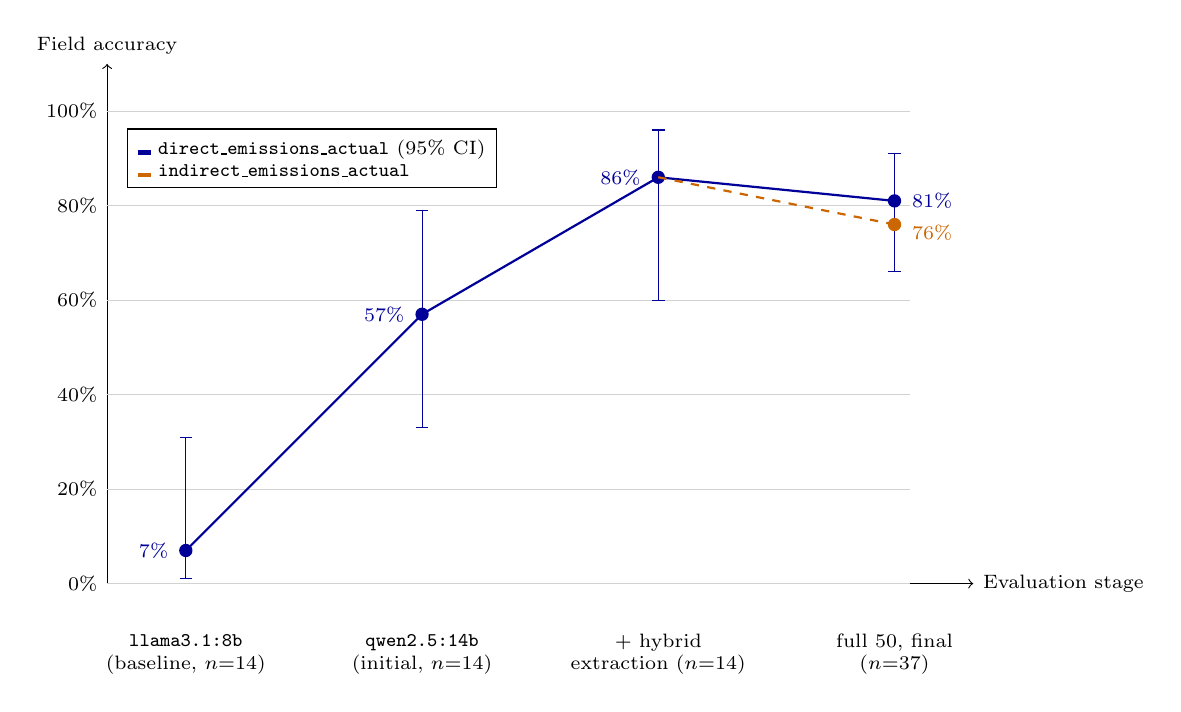
\begin{tikzpicture}[font=\small]
\draw[->] (0,0) -- (11,0) node[right, font=\scriptsize] {Evaluation stage};
\draw[->] (0,0) -- (0,6.6) node[above, font=\scriptsize] {Field accuracy};
\foreach \y/\lbl in {0/0\%, 1.2/20\%, 2.4/40\%, 3.6/60\%, 4.8/80\%, 6/100\%} {
  \draw[gray!35] (0,\y) -- (10.2,\y);
  \node[left, font=\scriptsize] at (0,\y) {\lbl};
}
\node[align=center, font=\scriptsize, text width=2.4cm] at (1,-0.9)
  {\texttt{llama3.1:8b}\\(baseline, $n$=14)};
\node[align=center, font=\scriptsize, text width=2.4cm] at (4,-0.9)
  {\texttt{qwen2.5:14b}\\(initial, $n$=14)};
\node[align=center, font=\scriptsize, text width=2.4cm] at (7,-0.9)
  {+ hybrid\\extraction ($n$=14)};
\node[align=center, font=\scriptsize, text width=2.6cm] at (10,-0.9)
  {full 50, final\\($n$=37)};
% 95% Wilson intervals, direct_emissions_actual
\foreach \x/\lo/\hi in {1/0.06/1.86, 4/1.98/4.74, 7/3.6/5.76, 10/3.96/5.46} {
  \draw[blue!60!black, thin] (\x,\lo) -- (\x,\hi);
  \draw[blue!60!black, thin] (\x-0.08,\lo) -- (\x+0.08,\lo);
  \draw[blue!60!black, thin] (\x-0.08,\hi) -- (\x+0.08,\hi);
}
\draw[thick, blue!60!black] (1,0.42) -- (4,3.42) -- (7,5.16) -- (10,4.86);
\foreach \x/\y/\v in {1/0.42/7, 4/3.42/57, 7/5.16/86} {
  \filldraw[blue!60!black] (\x,\y) circle (2.2pt);
  \node[left, font=\scriptsize, blue!60!black] at (\x-0.1,\y) {\v\%};
}
\filldraw[blue!60!black] (10,4.86) circle (2.2pt);
\node[right, font=\scriptsize, blue!60!black] at (10.1,4.86) {81\%};
\draw[thick, orange!80!black, dashed] (7,5.16) -- (10,4.56);
\filldraw[orange!80!black] (10,4.56) circle (2.2pt);
\node[right, font=\scriptsize, orange!80!black] at (10.1,4.46) {76\%};
\node[draw, fill=white, font=\scriptsize, align=left, inner sep=4pt]
  at (2.6,5.4) {\textcolor{blue!60!black}{\rule{1.5ex}{1.5pt}}~\texttt{direct\_emissions\_actual} (95\% CI)\\
  \textcolor{orange!80!black}{\rule{1.5ex}{1.5pt}}~\texttt{indirect\_emissions\_actual}};
\end{tikzpicture}
\vspace{0.4cm}
\caption{Accuracy on the two hardest fields across evaluation stages.}
\label{fig:accuracy_progression}
\end{figure}
\FloatBarrier

Figure~\ref{fig:accuracy_progression} summarises the trajectory on the two
fields that require genuine document comprehension. The two fields gave
identical results until the final full-50 run. The baseline and final
intervals ([1--31\%] and [66--91\%]) do not overlap, so the overall
improvement is not a small-sample artefact; the step between the last two
stages is within noise.

\subsection*{Raw Benchmark and Model Comparison}

The raw benchmark (Table~\ref{tab:benchmark_raw}) ran ten attempts per
model against the production argument-validation logic, scoring one tool
call per turn. Its two 0\% results were re-tested on the real harness, on
the same ten records (Table~\ref{tab:model_comparison}).

\begin{table}[H]
\centering
\setstretch{1.05}
\small
\renewcommand{\arraystretch}{1.15}
\begin{tabularx}{\textwidth}{|L{4.1cm}|L{2.4cm}|L{1.5cm}|X|}
\hline
\textbf{Model} & \textbf{Valid calls} & \textbf{Latency} & \textbf{Dominant failure mode} \\
\hline
\texttt{llama3.1:8b} & 5/10 [24--76\%] & 1.7\,s & Occasional invalid enum values \\
\hline
\texttt{qwen2.5:7b-instruct} & 4/10 [17--69\%] & 2.2\,s & Wrong argument types \\
\hline
\texttt{qwen3:8b} & 0/10 [0--28\%] & 14.1\,s & Several tool calls per turn \\
\hline
\texttt{qwen2.5:14b-instruct} & 0/10 [0--28\%] & 5.5\,s & Same multi-call pattern \\
\hline
\end{tabularx}
\caption{Raw tool-calling benchmark (95\% CI in brackets).}
\label{tab:benchmark_raw}
\end{table}
\FloatBarrier

\begin{table}[H]
\centering
\setstretch{1.05}
\small
\renewcommand{\arraystretch}{1.15}
\begin{tabularx}{\textwidth}{|L{4.1cm}|X|L{1.7cm}|L{1.9cm}|L{2.0cm}|}
\hline
\textbf{Model} & \textbf{Completed} & \textbf{Escalated} & \textbf{Exhausted} & \textbf{Field accuracy} \\
\hline
\texttt{llama3.1:8b} & 4/10 [17--69\%] & 5/10 & 1/10 & 12--30\% \\
\hline
\texttt{qwen2.5:7b-instruct} & 0/10 & 0/10 & 10/10 & 0\% \\
\hline
\texttt{qwen3:8b} & 8/10 [49--94\%] & 0/10 & 2/10 & 12--30\% \\
\hline
\end{tabularx}
\caption{Real-harness comparison on the same 10 records.}
\label{tab:model_comparison}
\end{table}
\FloatBarrier

The benchmark predicted that \texttt{qwen3:8b} could not complete a job
(0/10, interval [0--28\%]); on the real harness it completed 8/10
([49--94\%]). These intervals do not overlap, so the benchmark's verdict
was wrong for this system, not just unlucky. The comparison between
\texttt{qwen3:8b} and \texttt{llama3.1:8b} is weaker: 8/10 against 4/10
completed, with field accuracy identical, but the completion intervals
overlap, so ten records cannot separate the two models. The phase also
showed that prompt and architecture fixes closed the \textit{completion}
gap without moving \textit{accuracy} until the harness's own bugs were
fixed: finishing the loop and extracting the correct value have different
causes and different fixes.

\subsection*{From First Model to Final Configuration}

Table~\ref{tab:eval_stages} consolidates every later stage. ``Plumbing
fields'' are \texttt{quantity\_tonnes}, \texttt{data\_source} and
\texttt{precursor\_emissions}, which scored identically at every stage;
``comprehension fields'' are \texttt{direct\_emissions\_actual} and
\texttt{indirect\_emissions\_actual}, scored only on actual-sourced records.

\begin{table}[H]
\centering
\setstretch{1.05}
\footnotesize
\small
\renewcommand{\arraystretch}{1.2}
\begin{tabularx}{\textwidth}{|X|L{0.5cm}|L{1.8cm}|L{1.8cm}|L{1.8cm}|L{2.7cm}|}
\hline
\textbf{Stage} & \textbf{\textit{n}} & \textbf{Done / Esc. / Exh.} & \textbf{Plumbing fields} & \textbf{Carbon price} & \textbf{Comprehension} \\
\hline
1.~\texttt{llama3.1:8b}, fixed harness & 20 & 5 / 13 / 2 & 20\%\newline[8--42] & 15\% & 7\%\newline[1--31] \\
\hline
2.~\texttt{qwen2.5:14b-instruct} & 20 & 14 / 0 / 6 & 70\%\newline[48--85] & 60\%\newline[39--78] & 57\%\newline[33--79] \\
\hline
3.~+ hybrid regex/LLM extraction & 20 & 17 / 3 / 0 & 90\%\newline[70--97] & 70\%\newline[48--85] & 86\%\newline[60--96] \\
\hline
4.~Full 50 records & 50 & 34 / 14 / 2 & 68\%\newline[54--79] & 50\%\newline[37--63] & 73\% / 68\% \\
\hline
5.~+ fixture coverage (final) & 50 & 41 / 7 / 2 & \textbf{86\%\newline[74--93]} & \textbf{64\%\newline[50--76]} & \textbf{81\%\newline[66--91] / 76\%\newline[60--87]} \\
\hline
\end{tabularx}
\caption{Evaluation stages (95\% Wilson CI in brackets; comprehension is
direct / indirect where they differ).}
\label{tab:eval_stages}
\end{table}
\FloatBarrier

\textbf{Stage 1} ran after fixing several infrastructure bugs (missing
document context, an ORM constraint that made the default-value path
uncallable, an unset inference temperature, a value-carryover bug). The
comprehension fields barely moved, which motivated the source-quote
grounding gate. \textbf{Stage 2} switched to a larger model in the same
open-weight tier: every field improved, and comprehension rose from 7\%
to 57\%, the first evidence that the small-model ceiling was not
architectural. A re-run of \texttt{qwen3:8b} with the full safeguard set
(16/20 completed, 25--35\% on plumbing fields, 7\% on comprehension)
confirmed the gap, and also exposed an instrumentation bug: the
reasoning-turn counter read zero because the model returned its reasoning
in a separate \texttt{message.reasoning} field. Once fixed, reasoning
appeared on effectively every turn. \texttt{qwen2.5:14b-instruct} became
the default model.

\textbf{Stage 3} added the regex pre-parser to \texttt{extract\_field}.
Two regressions were caught before any aggregate was trusted: a generic
result shape that the model copied into the write call, silently zeroing
every value, and a null-coercion fix that zeroed a correctly extracted
sibling value. This is the strongest result measured, but it targets the
dataset's own templates; a document in an unfamiliar format falls back to
plain LLM reading.

\textbf{Stage 4} ran the full 50 records for the first time. Records 20--49,
never used during development, scored well below records 0--19 (plumbing
53\% against 90\%). Table~\ref{tab:full50_mechanisms} lists the three
causes, each traced live on individual records.

\begin{table}[H]
\centering
\setstretch{1.05}
\small
\renewcommand{\arraystretch}{1.15}
\begin{tabularx}{\textwidth}{|L{3.2cm}|X|L{2.6cm}|}
\hline
\textbf{Cause} & \textbf{Evidence} & \textbf{Status} \\
\hline
Test-fixture gap & Default-factor fixtures covered 6 of the 13 (sector, route, country) combinations; 7 of 11 escalations in records 20--49 needed a missing one, and the model correctly escalated & Fixed (stage 5) \\
\hline
Single write vs.\ grounding gate & The gate rejected a fabricated direct value three times; the model escalated, and the correctly extracted indirect value was discarded with it & Design trade-off, open \\
\hline
Run-to-run variance & Two records scored zero in the batch but were fully correct when re-run on the same code (temperature~0.1) & Model property \\
\hline
\end{tabularx}
\caption{Causes of the lower full-50 score.}
\label{tab:full50_mechanisms}
\end{table}
\FloatBarrier

\textbf{Stage 5} extended the fixtures to all 13 combinations. Escalations
in records 20--49 fell from 11 to 4, exactly the 7 records the diagnosis
predicted. The plumbing-field gain (68\% to 86\%) is at the edge of the
intervals; the comprehension gains (73\% to 81\%, 68\% to 76\%) are within
noise and are reported as observed only.

\subsection*{Self-Consistency (Rejected) and Two Targeted Fixes}

Self-consistency, sampling several answers and taking the majority, is a
standard way to reduce random reasoning errors~\cite{wang2023selfconsistency}.
It was tested on 15 records with two independent runs each: 13 were
correct both times, 2 were wrong both times with the same failure, and
none disagreed. Majority voting only helps when a second draw can avoid an
error, and every failure observed here was systematic, so it would have
doubled cost for no measured benefit. Zero disagreements in 15 still
leaves a true disagreement rate of up to 20\% plausible, so the
rejection is a judgement for this scale, not a proof. The two systematic
failures were instead traced and fixed. First, the model sometimes never
asked for \texttt{carbon\_price\_paid\_origin}; the dispatcher now parses
that field opportunistically whenever \texttt{extract\_field} runs. Second,
on a customs document with no emissions data, the model spent all nine
iterations retrying a write; a prompt rule now makes it escalate, which it
did in 3 iterations. On records 0--19, carbon price rose from 70\% to 80\%
(14/20 to 16/20, intervals overlapping) and no other field changed. These
two fixes have not yet been re-run on all 50 records.

\subsection*{Summary Metrics}

\begin{table}[H]
\centering
\setstretch{1.05}
\small
\renewcommand{\arraystretch}{1.1}
\begin{tabularx}{\textwidth}{|L{6.4cm}|X|}
\hline
\textbf{Metric} & \textbf{Value} \\
\hline
Development window & 2026-07-28 $\rightarrow$ 2026-09-18 \\
\hline
Commits / automated tests & 66 / 175 test functions in 14 files \\
\hline
Python lines of code & $\approx$7{,}600 incl.\ tests ($\approx$4{,}400 application) \\
\hline
Odoo models / agent tools / candidate LLMs & 9 / 7 / 4 \\
\hline
Default model & \texttt{qwen2.5:14b-instruct} \\
\hline
Plumbing fields, full 50 (final) & 64--86\% (lowest field 64\% [50--76]) \\
\hline
Comprehension fields, full 50 (final) & 76--81\% ([60--87], [66--91]) \\
\hline
\end{tabularx}
\caption{Project summary metrics.}
\label{tab:summary_metrics}
\end{table}
\FloatBarrier

% ─────────────────────────────────────────────
\section{Limitations and Threats to Validity}
\label{sec:limitations_cbam}

Table~\ref{tab:limitations} lists what the results above do and do not
support. The first four rows concern how far the numbers generalise; the
rest are open engineering items.

\begin{table}[H]
\centering
\setstretch{1.05}
\small
\renewcommand{\arraystretch}{1.15}
\begin{tabularx}{\textwidth}{|L{3.4cm}|X|L{3.4cm}|}
\hline
\textbf{Limitation} & \textbf{Consequence} & \textbf{What would close it} \\
\hline
Small sample (10--50 records) & Intervals are wide; only the baseline-to-final gain and the benchmark reversal are clearly outside noise & A larger evaluation set \\
\hline
Synthetic data only & Documents come from templates the regex pre-parser was built for, so accuracy on real supplier paperwork is unmeasured & Even 10--20 real certificates \\
\hline
Narrow model range & Four open-weight 7--14B models (Llama, Qwen), all served through Ollama; larger or hosted models were not tested & Broader model sweep \\
\hline
No single-shot baseline & The agentic loop was not compared with one extraction call per document on the same harness, so its benefit is argued, not measured & Ablation run on the LLM host \\
\hline
Not production-grade & Final run: 7/50 escalate, 2/50 exhaust the cap, no field reaches 100\% & Further fixes, human review \\
\hline
Single write vs.\ grounding gate & A rejected fabrication discards a correctly extracted sibling value on the same record & Partial writes, design change \\
\hline
Two fixes on 20 records only & Carbon-price recovery and the customs prompt rule are unvalidated at full scale (full-50 figure: 64\%) & Full-50 re-run \\
\hline
Value carry-over & The model once replaced a looked-up factor with invented numbers; dispatcher memory mitigates the symptom, not the behaviour & Model or prompt change \\
\hline
Deployment unverified & The two-machine topology runs on a VPN workaround and has not been verified end to end; the LLM host has not been run against the physical Odoo deployment & Live two-machine test \\
\hline
Reasoning vs.\ correctness & Reasoning-turn counts are now measured but not yet correlated with correct extractions & Analysis over a full run \\
\hline
\end{tabularx}
\caption{Limitations and threats to validity.}
\label{tab:limitations}
\end{table}
\FloatBarrier

% ─────────────────────────────────────────────
\section{Conclusion}

This chapter has shown the three design principles of
Chapter~\ref{chap:design} realised concretely: an independently tested
calculation engine that no language model ever writes to directly, a
tool-use loop with no hardcoded ordering logic, and a benchmarking
methodology rigorous enough to catch and correct its own initial ranking
error --- twice over, first correcting a wrongly-dismissed
\texttt{qwen3:8b}, then discovering and adopting the stronger
\texttt{qwen2.5:14b-instruct}. Applied to synthetic CBAM declarations for
steel and aluminium, and measured honestly at full dataset scale rather
than on a flattering subsample, the system raised measured field
accuracy from a 0\% baseline to 64--86\% on plumbing-reachable fields and
76--81\% on document-comprehension fields. Those were the fields this
project's evaluation history had treated as a hard model-capability
ceiling, until a larger model and a hybrid deterministic/LLM extraction
path together showed that ceiling was not architectural after all. What
remains open is not whether the architecture works, but how far its two
still-unresolved tradeoffs --- the single-write/grounding-gate
interaction, and two fixes not yet re-validated at full scale --- can be
closed without reintroducing the risks Chapters~\ref{chap:context}
and~\ref{chap:design} were designed to rule out.
